\chapter{Bäume in der Informatik}
\label{chap:kapitel2}

\section{Definition von Bäumen}

Nach Wetherell und Shannon sind Bäume endliche, gerichtete, zusammenhängende, azyklische Graphen \cite[S.515]{q1}. 
Bäume bestehen lediglich aus zwei Elementen, nämlich den Knoten und den Kanten. Die Kanten sind gerichtet und verbinden die einzelnen 
Knoten miteinander. Dabei hat jeder Knoten maximal einen Vorgänger, welcher als Vater bezeichnet wird, und null 
bis n viele Nachfolger, welche Kinder genannt werden. Die Wurzel stellt hierbei einen besonderen Knoten dar, da sie der 
einzige Knoten ohne Vorgänger ist. Zudem besitzt jeder Knoten eine Höhe. Diese Höhe ist definiert als die Anzahl an Kanten zwischen dem
Knoten und der Wurzel \cite[S.515]{q1}. Außerdem kann jeder Knoten Daten beinhalten. Eine weitere besondere Form von Knoten sind die Blätter. 
Diese verfügen über keine Kinder \cite[S.4]{q4}. Abbildung \ref{pic:simple_tree} zeigt einen einfachen Binärbaum.

\begin{figure}[H]
    \centering
    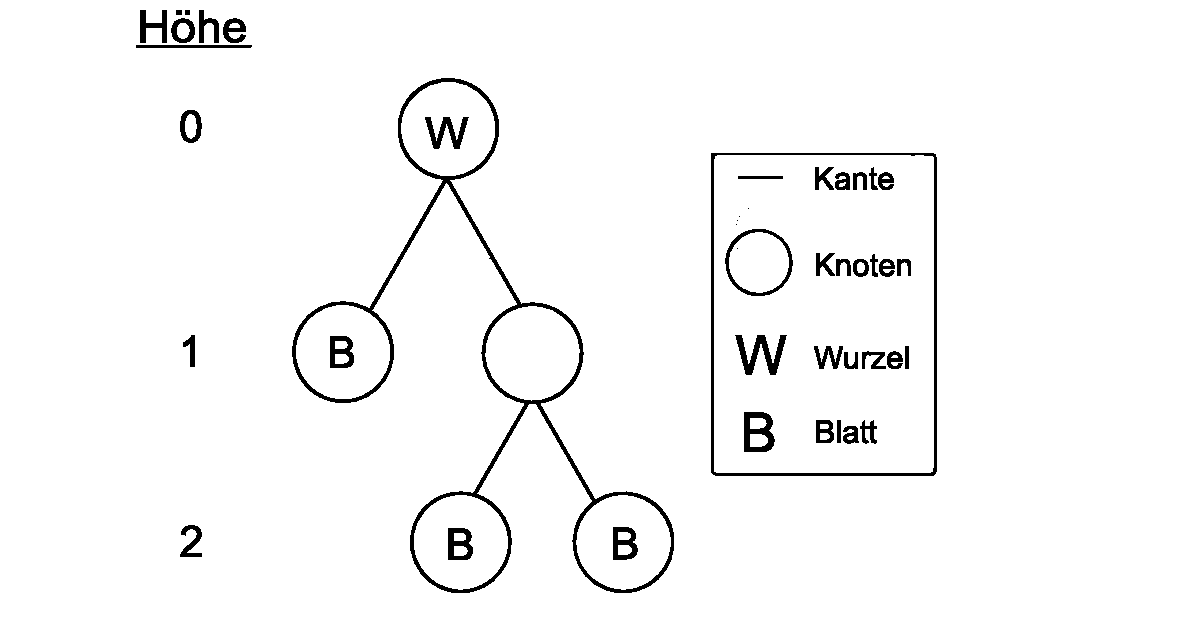
\includegraphics[scale = 0.5]{abbildungen/simple_tree}
    \caption{Einfacher beschrifteter Binärbaum}
    \label{pic:simple_tree} 
\end{figure}

Eine spezielle Form von Bäumen stellen die sogenannten Binärbäume dar. 
Binärbäume sind Bäume, wo jeder Knoten maximal zwei Kinder hat.

Um jeden Knoten eines Baumes abarbeiten zu können, kann über dem Baum 
traversiert werden. Traversierung bezeichnet das systematische Ablaufen 
von jedem Knoten eines Baumes beginnend bei der Wurzel. Eine Möglichkeit dazu ist die sogenannte
Pre-Order-Traversierung. Dabei wird zunächst der Knoten, dann der linke Teilbaum
und zum Schluss der rechte Teilbaum besucht. Hier werden die Väter vor den
Kindern durchlaufen. Eine weitere Möglichkeit zur Traversierung ist die 
Post-Order-Traversierung. Dabei wird als erstes der linke Teilbaum, dann der 
rechte Teilbaum und dann der Knoten besucht \cite[S.22]{q4}. Bei dieser Art der 
Traversierung werden die Kinder vor den Väter durchlaufen. Neben diesen Arten
der Traversierung gibt es noch weitere Möglichkeiten, wie über einem 
Baum traversiert werden kann. Diese sind für das Verständnis der hier 
vorgestellten Algorithmen aber nicht notwendig.


\section{Anwendungsgebiete}

Bäume erfahren einen vielfältigen Einsatz in der Informatik, zum Beispiel 
als Datenstruktur, als Syntaxbäume, als Ausdrucksbäume oder auch als 
Entscheidungsbäume.

Ein Baum als Datenstruktur kann beispielsweise dazu verwendet werden, 
um eine Menge von Daten zu sortieren oder in ihnen effizient nach einen 
bestimmten Datensatz zu suchen. So verwendet der Heap-Sort-Algorithmus 
einen Baum zum Sortieren von Daten. Ebenso können Bäume, in Form von Syntaxbäumen, dazu verwendet 
werden, um Syntaxregeln zu überprüfen. Zudem werden Bäume verwendet, um mathematische 
Ausdrücke auszuwerten. Hierfür wird ein sogenannter Ausdrucksbaum für einen 
gegebenen mathematischen Ausdruck aufgestellt und ausgewertet. In der 
Datenanalyse werden Bäume in Form von Entscheidungsbäumen verwendet. 
Diese werden benutzt um Abhängigkeiten darzustellen. Die Knoten des Baumes stellen in diesem Fall Attribute dar und die Kanten des Knotens
die verschiedenen Ausprägungen des Attributs. Die Blätter stellen die vorhergesagten Kategorien dar. So können beispielsweise neue 
Datensätze, in Abhängigkeit zu ihren Werten, einer bestimmten Kategorie 
zugeordnet werden.

Wie schon angekündigt, werden Bäume auch außerhalb der Informatik häufig verwendet. Sie können 
dazu genutzt werden um zum Beispiel eine Hierarchie eines Unternehmens
dazustellen oder einen Stammbaum einer 
Familie wie in der Abbildung \ref{pic:stammbaum} \cite[S.2]{q4}.

\begin{figure}[h]
    \centering
    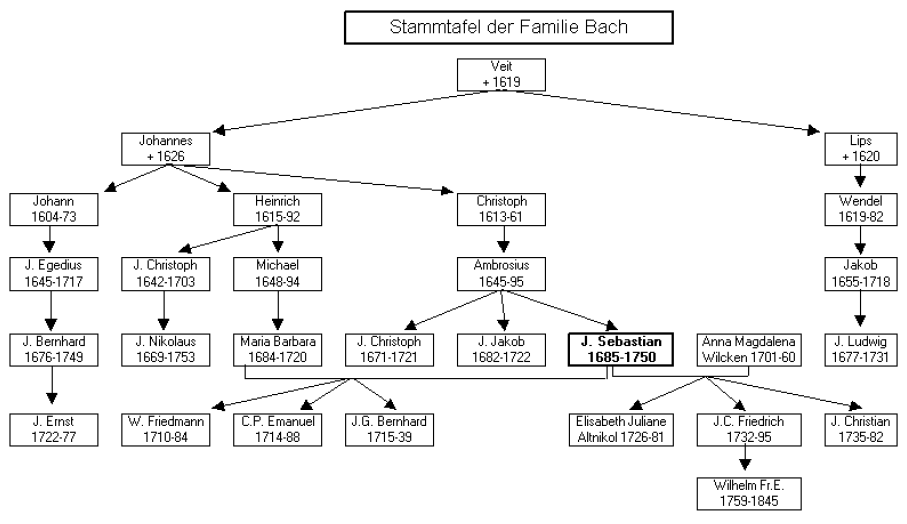
\includegraphics[scale=0.7]{abbildungen/Stammbaum.png}
    \caption{Ein Stammbaum, Beispiel für Bäume als Datenstrukturen \cite[]{q4}}
    \label{pic:stammbaum}
\end{figure}
